%% LyX 2.0.3 created this file.  For more info, see http://www.lyx.org/.
%% Do not edit unless you really know what you are doing.
\documentclass[oneside,spanish]{book}
\usepackage[T1]{fontenc}
\usepackage[latin9]{inputenc}
\usepackage{listings}
\usepackage[a4paper]{geometry}
\geometry{verbose,tmargin=2cm,bmargin=3cm,lmargin=2cm,rmargin=2cm}
\setcounter{secnumdepth}{3}
\setcounter{tocdepth}{3}
\usepackage{amsmath}
\usepackage{graphicx}

\makeatletter

%%%%%%%%%%%%%%%%%%%%%%%%%%%%%% LyX specific LaTeX commands.
%% Because html converters don't know tabularnewline
\providecommand{\tabularnewline}{\\}

%%%%%%%%%%%%%%%%%%%%%%%%%%%%%% Textclass specific LaTeX commands.
\newenvironment{lyxcode}
{\par\begin{list}{}{
\setlength{\rightmargin}{\leftmargin}
\setlength{\listparindent}{0pt}% needed for AMS classes
\raggedright
\setlength{\itemsep}{0pt}
\setlength{\parsep}{0pt}
\normalfont\ttfamily}%
 \item[]}
{\end{list}}

%%%%%%%%%%%%%%%%%%%%%%%%%%%%%% User specified LaTeX commands.
\usepackage[T1]{fontenc}
\usepackage[latin9]{inputenc}
\usepackage{listings}
\usepackage[spanish]{babel}
\usepackage{times}

\usepackage{color}
\definecolor{javared}{rgb}{0.6,0,0} % cadenas
\definecolor{javagreen}{rgb}{0.25,0.5,0.35} % comentarios
\definecolor{javapurple}{rgb}{0.5,0,0.35} % palabras clave
\definecolor{javadocblue}{rgb}{0.25,0.35,0.75} % javadoc :D

\lstset{language=C++,
basicstyle=\ttfamily,
frame=single,
keywordstyle=\color{javapurple}\bfseries,
stringstyle=\color{javared},
commentstyle=\color{javagreen},
morecomment=[s][\color{javadocblue}]{/**}{*/},
numbers=left,
numberstyle=\small\color{black},
numbersep=10pt,
tabsize=4,
showspaces=false,
showstringspaces=false,
breaklines=true}

\makeatother

\usepackage{babel}
\addto\shorthandsspanish{\spanishdeactivate{~<>}}

\begin{document}
\tableofcontents{}


\chapter{Ad-hoc}


\section{Invertir Bytes}

\lstinputlisting{adhoc/utilidades.cpp}


\section{A�o bisiesto}

\lstinputlisting{adhoc/bisiesto.cpp}


\section{Doomsday}

\lstinputlisting{adhoc/doomsday.cpp}


\section{Hanoi}

\lstinputlisting{utilitarios/hanoi.cpp}


\chapter{Estructuras}


\section{Union - Find}

\lstinputlisting{estructuras/unionfind.cpp}


\section{BIT}

\lstinputlisting{estructuras/bit.cpp}


\section{Segment Tree}

\lstinputlisting{estructuras/SegmentTree2.cpp}

Otra implementacion en java:

\lstinputlisting{estructuras/SegmentTree.java}


\section{Segment Tree con Lazy Propagati�n}

\lstinputlisting{estructuras/SegmenTree_lazy.cpp}


\section{Trie}

\lstinputlisting{estructuras/trie.cpp}


\section{Arbol Binario de Busqueda}

\lstinputlisting{estructuras/arbolbinario.cpp}


\chapter{Complete Search }


\section{El problema de las ocho reinas}

\lstinputlisting{busquedacompleta/ochoreinas.cpp}


\section{El problema de las ocho reinas acelerado con Bits}

\lstinputlisting{busquedacompleta/ochoreinas2.cpp}


\chapter{Divide y venceras}


\section{Busqueda Binaria (Recursivo)}

\lstinputlisting{divideyvenceras/busquedabinariarecursivo.cpp}


\section{Busqueda Binaria (Iterativo)}

\lstinputlisting{divideyvenceras/busquedabinariaiterativo.cpp}


\section{MergeSort}

Primera implementacion:

\lstinputlisting{divideyvenceras/mergesort.cpp}

Segunda implementaci�n:

\lstinputlisting{divideyvenceras/mergesort2.cpp}


\section{Meet in the Middle}

Si generamos los subconjuntos de una lista de N elementos; sabemos
que existen 2N subconjuntos, pero esta complejidad es demasiado cuando
N es grande, digamos (N>20).

Problema.- Dado una secuencia de N (1<= N <=34) n�meros, determinar
cu�ntos subconjuntos de esta secuencia tiene una suma entre A y B.

Esta t�cnica consiste en \emph{dividir en dos listas por la mitad},
Luego generamos las sumatorias de los subconjuntos de cada lista y
\emph{los ordenamos}. Luego combinar ambos resultados.

Considerare la sumatoria de conjunto vacio como 0.


\subsubsection*{Ejemplo:}

L= \{ 2 , 5 , 6 , 1, 9\};

A=5, B=15

\textbf{Los dividimos en los listas por la mitad.}

X= \{ 2 , 5, 6\}

Y= \{ 1 , 9\}

\textbf{Generamos los subconjuntos de cada lista.}

X\textquoteright{} = \{ 0, 2, 5 , \{2,5\}, 6,\{2,6\}, \{5,6\} ,\{2,5,6\}
\}

Y\textquoteright{}= \{ 0, 1, 9, \{1,9\} \}

\textbf{Sumatorias de cada subconjunto de manera ordenada.}

X\textquoteright{}= \{0,2,5,6,7,8,11,13\}

Y\textquoteright{}= \{0,1,9,10\}

\textbf{Combinar resultados}

Tenemos que recorrer la lista X\textquoteright{} y ver cu�nto nos
falta para llegar al intervalo {[}A, B{]}.
\begin{itemize}
\item Si el primer elemento de X\textquoteright{} tenemos 0 entonces en
la lista Y\textquoteright{} tenemos que buscar cuantos elementos existen
entre 5 y 15.
\item Si el segundo elemento de X\textquoteright{} tenemos 2 entonces en
la lista Y\textquoteright{} buscamos cuantos existen entre 3 y 13.
\end{itemize}
x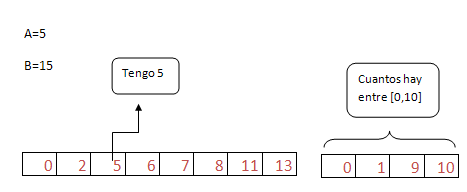
\includegraphics[scale=0.7]{imagenes/meet}

Si bien se dan cuenta es muy importante tener ambas listas de una
manera ordenada para poder buscar cuantos elementos existen en la
segunda matriz entre ese intervalo.

El algoritmo sigue buscando hasta terminar con el �ltimo elemento
de la primera lista.

\lstinputlisting{divideyvenceras/meetinthemiddle.cpp}


\chapter{Programaci�n Dinamica}


\section{El problema de la mochila y Subset Sum}


\subsubsection*{Subset Sum:}

$OPT(j,W)=max\begin{cases}
OPT(j-1,W) & (w_{j}>W)\\
w_{j}+OPT(j-1,W-w_{j}) & (w_{j}\leq W)
\end{cases}$


\subsubsection*{0-1 Mochila}

$OPT(j,W)=max\begin{cases}
OPT(j-1,W) & (w_{j}>W)\\
\mathbf{v_{j}}+OPT(j-1,W-w_{j}) & (w_{j}\leq W)
\end{cases}$

\lstinputlisting{programaciondinamica/mochila.cpp}


\section{El problema de la mochila(iterativo)}

\lstinputlisting{programaciondinamica/mochilaiterativo.cpp}


\section{Cambio de modenas}

\lstinputlisting{programaciondinamica/coin_change.cpp}


\section{LIS ($O(n^{2})$)}

\lstinputlisting{programaciondinamica/lis1.cpp}


\section{LIS ($O(n\, log(n)$)}

\lstinputlisting{programaciondinamica/lis2.cpp}


\section{Suma maxima en rango}

\lstinputlisting{programaciondinamica/max1drangesum.cpp}


\section{Suma maxima en rango 2D $O(n^{4})$}

\lstinputlisting{programaciondinamica/max2drangesum1.cpp}


\section{Suma maxima en rango 2D $O(n^{3})$}

\lstinputlisting{programaciondinamica/max2drangesum2.cpp}


\section{Maxima submatriz de ceros}

\lstinputlisting{programaciondinamica/maximasubmatrizceros.cpp}


\section{Submatriz de suma maxima}

\lstinputlisting{programaciondinamica/sumamaxima.cpp}


\section{Distancia de edici�n (Algoritmo de Levenshtein)}

\lstinputlisting{programaciondinamica/levenshtein.cpp}


\section{Distancia de edici�n (Recursivo)}

\lstinputlisting{programaciondinamica/editdistance.cpp}


\chapter{Grafos}


\section{BFS}

\lstinputlisting{grafos/bfs.cpp}


\section{DFS}

\lstinputlisting{grafos/dfs_ff.cpp}


\section{Topological Sort}

Grafo Aciclico Dirigido (DAG) 

Las tareas no son independientes y la ejecuci�n de una tarea s�lo
es posible si otras tareas que ya se han ejecutado. Solo hay un orden 

\lstinputlisting{grafos/TopSort.cpp}


\section{Dijkstra}

\lstinputlisting{grafos/dijkstra.cpp}


\section{BellmandFord}

Si un grafo contiene un ciclo de coste total negativo entonces este
grafo no tiene soluci�n

\lstinputlisting{grafos/bellmandford.cpp}


\section{Floyd Warshall}

\lstinputlisting{grafos/FloydWarshall.cpp}


\section{Componentes Fuertemente Conexas }

\lstinputlisting{grafos/scc.cpp}


\section{Componentes Fuertemente Conexas (Kosaraju)}

\lstinputlisting{grafos/Kosaraju.cpp}


\section{Componentes Fuertemente Conexas (Tarjan $O(n+v)$ )}

\lstinputlisting{grafos/Tarjan.cpp}

Otra implementacion:

\lstinputlisting{grafos/tarjan2.java}


\section{Minimum Spanning Tree (Kruskall)}

\lstinputlisting{grafos/kruskall.cpp}


\section{Second Minimum Spanning Tree}

Segundo Mejor Arbol de Expansion Complejidad: O(V{*}E) , (V = nodos,
E=Arcos)
\begin{itemize}
\item Armamos el primer MST 
\item Para cada arco en el MST el Segundo Mejor Arbol de Expansion es el
minimo de: 

\begin{itemize}
\item Ignoramos ese arco 
\item Hallamos el MST sin ese arco 
\end{itemize}
\item No es necesario volver a ordenar por que ya se ordeno al calcular
el primer MST
\end{itemize}
\lstinputlisting{grafos/segundomst.cpp}


\section{Minimum Cut}

\lstinputlisting{grafos/MinCut.cpp}


\section{MaxFlow}

\lstinputlisting{grafos/MaxFlow.cpp}


\section{Lowest common ancestor (LCA)}

\lstinputlisting{grafos/LCA.cpp}


\section{Maximo Emparejamiento Bipartito }

\lstinputlisting{grafos/MaximoEmparejamientoBipartito.cpp}


\section{Puentes}

\lstinputlisting{grafos/bridges.java}


\section{Puntos de Articulaci�n}

\lstinputlisting{grafos/ArticulationPoints.java}


\section{Camino Euleriano}

\lstinputlisting{grafos/eulertour.cpp}


\section{Dijkstra Fast}

\lstinputlisting{grafos/dijkstrafast.cpp}


\chapter{Matem�ticas}


\section{GCD}

\lstinputlisting{matematicas/gcd.cpp}


\section{LCM}

\lstinputlisting{matematicas/lcm.cpp}


\section{Algoritmo extendido de euclides}

\lstinputlisting{matematicas/euclidesextendido.cpp}


\section{Exponenciaci�n rapida}

\lstinputlisting{matematicas/exponenciacion.cpp}


\section{Criba de Erathostenes}

\lstinputlisting{matematicas/criba.cpp}


\section{Criba de Erathostenes Aumentada}

\lstinputlisting{matematicas/cribaaumentada.cpp}


\section{Triangulo de Pascal}

\lstinputlisting{matematicas/pascal.cpp}


\section{Combinaciones(Para numeros muy grandes)}

\lstinputlisting{matematicas/combinaciones.cpp}


\section{Polinomios}

\lstinputlisting{matematicas/Polinomio.java}


\section{Fibonacci ( $O(log(n))$ )}

\lstinputlisting{matematicas/fibonacci.cpp}


\section{Multiplicaci�n entero por cadena}

\lstinputlisting{matematicas/multiplicacion.cpp}


\section{Multiplicaci�n de numeros grandes (Karatsuba)}

\lstinputlisting{matematicas/karatsuba.java}


\section{Integracion de Simpson}

\lstinputlisting{matematicas/integracion.cpp}


\section{Inverso modular}

Si queremos hallar $a/b(mod\, p)$ donde $p$ es $primo$, es lo mismo
que:

$(a*b^{-1})(mod\, p)$

donde $b^{-1}$ es el inverso modular de $b$ .

Para hallar el inverso modular de un numero $x$modulo $p$: 

$x^{-1}(mod\, p)=modpow(x,p-2,p)$ 

Entonces, volviendo al problema:

$a/b(mod\, p)=(a*modpow(b,p-2,p)%)%p
$


\section{El juego de Nim}

\lstinputlisting{matematicas/nim.cpp}


\section{Fraccion}

\lstinputlisting{matematicas/fraccion.cpp}


\section{Matriz}

\lstinputlisting{matematicas/matrix.cpp}


\section{Gauss Jordan}

\lstinputlisting{matematicas/gaussjordan.cpp}


\section{Numeros romanos}

\lstinputlisting{matematicas/romanos.cpp}


\chapter{Cadenas}


\section{Utilidades}

\lstinputlisting{cadenas/utilidades.cpp}


\section{Boyer Moore}

Encuentra todos los match de un patron en el texto.

\lstinputlisting{cadenas/boyerMoore.cpp}


\section{Knuth Morris Pratt }

\lstinputlisting{cadenas/kmp.cpp}


\section{Iesima permutaci�n}

\lstinputlisting{cadenas/ipermutacion.cpp}


\section{Algoritmo de Manacher}

El algoritmo guarda el tama�o del palindrome mas grande en LP{[}pos{]}
que tiene como centro las posici�n \emph{pos} en la cadena original

\lstinputlisting{cadenas/manacher.cpp}

Otra implementacion:

\lstinputlisting{cadenas/manacher2.cpp}


\section{Longest Common Subsequence (LCS)}

\lstinputlisting{cadenas/lcs.cpp}


\section{Suffix Array}

\lstinputlisting{cadenas/sa.cpp}


\section{Suffix Array DC3}

\lstinputlisting{cadenas/dc3_sybcadena.cpp}


\section{Minima Rotacion Lexicografica}

\lstinputlisting{cadenas/MinRotLex.cpp}


\section{Trie}

\lstinputlisting{cadenas/trie.cpp}


\section{Aplicaciones}

\lstinputlisting{cadenas/aplicaciones.txt}


\chapter{Geometria Computacional}


\section{Intersecci�n de rectangulos}

\lstinputlisting{geometria/interseccionrect.cpp}


\section{Distancia Punto - Segmento}

\lstinputlisting{geometria/puntosegmento.cpp}


\section{Distancia Punto - Recta}

\lstinputlisting{geometria/puntorecta.cpp}


\chapter{Utilitarios}


\section{Plantilla}

\lstinputlisting{utilitarios/plantilla.cpp}


\section{Lectura rapida}

\lstinputlisting{utilitarios/entrada.cpp}


\section{Espicificadores de formato para printf y scanf}

\begin{tabular}{|c|c|}
\hline 
\textbf{Especificador} & \textbf{Tipo}\tabularnewline
\hline 
\hline 
\%c & char\tabularnewline
\hline 
\%s & cadena\tabularnewline
\hline 
\%d, \%i & int\tabularnewline
\hline 
\%u & unsigned int\tabularnewline
\hline 
\%ld & long int\tabularnewline
\hline 
\%lu & unsigned long int\tabularnewline
\hline 
\%lld & long long int\tabularnewline
\hline 
\%llu & unsigned long long int\tabularnewline
\hline 
\%e, \%f, \%g & float\tabularnewline
\hline 
\%lf & double\tabularnewline
\hline 
\%o & n�mero octal\tabularnewline
\hline 
\%x & n�mero hexadecimal\tabularnewline
\hline 
\%patron & patron\tabularnewline
\hline 
\end{tabular}


\section{Contar bits en 1 en un numero}

\textbf{C++ :}

\begin{lstlisting}
__builtin_popcount(unsigned int)
__builtin_popcountll(unsigned long long)
\end{lstlisting}


\textbf{Java : }

\begin{lstlisting}
Integer.bitCount(int) 
\end{lstlisting}



\section{Busqueda binaria}

C++'s Standard Template Library has four functions for binary search,
depending on what information you want to get. They all need 
\begin{lyxcode}
\#include~<algorithm>~
\end{lyxcode}
The \textbf{lower\_bound()} function returns an iterator to the first
position where a value could be inserted without violating the order;
i.e. the first element equal to the element you want, or the place
where it would be inserted.
\begin{lyxcode}
int~{*}ptr~=~std::lower\_bound(array,~array+len,~what);~

//~a~custom~comparator~can~be~given~as~fourth~arg
\end{lyxcode}
The \textbf{upper\_bound()} function returns an iterator to the last
position where a value could be inserted without violating the order;
i.e. one past the last element equal to the element you want, or the
place where it would be inserted.
\begin{lyxcode}
int~{*}ptr~=~std::upper\_bound(array,~array+len,~what);~

//~a~custom~comparator~can~be~given~as~fourth~arg
\end{lyxcode}
The \textbf{equal\_range()} function returns a pair of the results
of lower\_bound() and upper\_bound().
\begin{lyxcode}
std::pair<int~{*},~int~{*}>~bounds~=~std::equal\_range(array,~array+len,~what);~

//~a~custom~comparator~can~be~given~as~fourth~arg
\end{lyxcode}
Note that the difference between the bounds is the number of elements
equal to the element you want.

The \textbf{binary\_search()} function returns true or false for whether
an element equal to the one you want exists in the array. It does
not give you any information as to where it is.
\begin{lyxcode}
bool~found~=~std::binary\_search(array,~array+len,~what);~

//~a~custom~comparator~can~be~given~as~fourth~arg\end{lyxcode}

\end{document}
